%----------------------------------------
% Preamble to set up the document
%----------------------------------------
\documentclass{article}

% set up packages (you shouldn't need to touch this)
\usepackage{graphicx}  % required to insert images
\usepackage{hyperref}  % for hyperlinks
\usepackage[svgnames]{xcolor}  % to change hyperlink colors
\colorlet{linkcolour}{DarkBlue}
\hypersetup{colorlinks=true, linkcolor=linkcolour, citecolor=linkcolour, urlcolor=linkcolour,}

% Margins
\topmargin=-0.45in
\evensidemargin=0in
\oddsidemargin=0in
\textwidth=6.5in
\textheight=9.0in
\headsep=0.25in

% use a sans serif font
\renewcommand{\familydefault}{\sfdefault}

%----------------------------------------
% Step 1: Edit the lecture title
%----------------------------------------
\title{
Lecture 7: Regression II: Theory and Practice \\  % Lecture title
Modeling Social Data, Spring 2017 \\   % Course title
Columbia University                    % School
}

%----------------------------------------
% Step 2: Edit your name and the date
%----------------------------------------
\author{Harsha Vemuri}                     % Scribe's name
\date{March 3, 2017}                % Lecture date

\begin{document}

\maketitle


%----------------------------------------
% Step 3:
% Rename uni.tex to match your uni,
% edit the filename accordingly below,
% and put your notes in this file
%----------------------------------------
%----------------------------------------
% Write your notes here
%----------------------------------------

\section{How to Evaluate Models}

We try to find the best parameters by inspecting the fit of the model:
\begin{enumerate}
\item Plot the actual and model-predicted values 
\item Break this down using a different color for each gender
\item We can also color by age and wrap by gender for clarity
\end{enumerate}

\section{Modeling Variability}

This is done by summarizing the average of each gender-age combo, which causes us to overlook variability in the observations. Plotting every point shows variability in age is greater than variability across age, revealing issues with the model. 

\begin{figure}[h]
\begin{center}
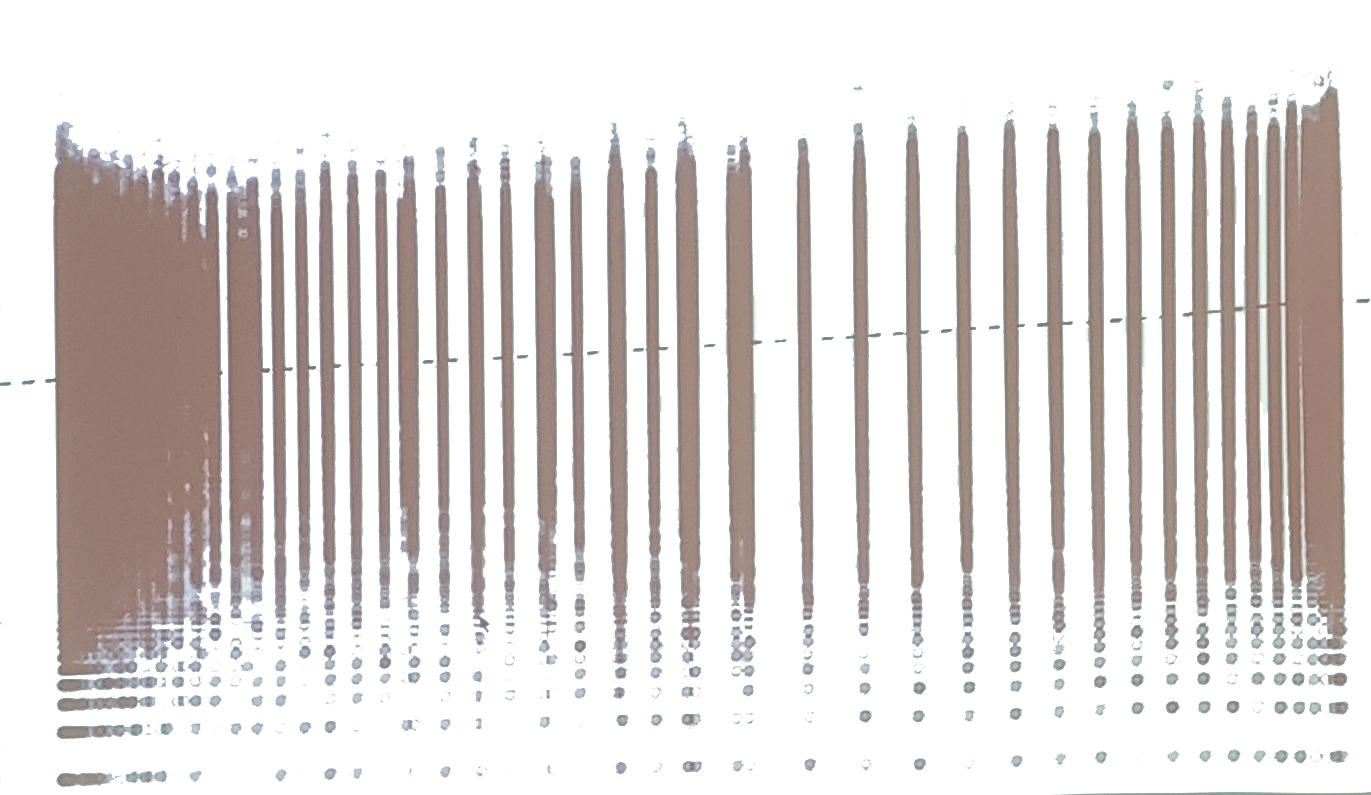
\includegraphics[width=0.5\textwidth]{figures/figure1.jpg}
\caption{Observations Plot}
\end{center}
\end{figure}

Traditional methods of reporting statistics by significance overlook this variability as well. We can thus explain overall trends, but not individual observations that may be seen. There may also be unexplored transformations that could reduce variability, or other confouding variables that affect the parameters but have not necessarily been recorded via the model. 

\section{How Good is a Model?}

There are two metrics used to evaluate a model's fit:
\begin{itemize}
\item RMS (root-mean-squared) error (equation below)
\item Pearson's Correlation Coefficient (equation below)
\end{itemize}

RMSE = $\sqrt{\frac{1}{N}\sum_{i}^{N}(y_i-\hat{y})^2}$ \\ 
Pearson's r = $\frac{\sum_i(y_i-\bar{y})(\hat{y_i}-\hat{\bar{y}})}{[\sum_i(y_i-\bar{y})^2]^\frac{1}{2}[\sum_i(\hat{y_i}-\hat{\bar{y}})^2]^\frac{1}{2}}$ \\ \\ 

Note that the square of the Pearson coefficient is the $R^2$ of the model, the fraction of variance explained. 

\section{Explaining the Past vs. Predicting the Future}

Adding degrees to a polynomial model adds accuracy to its predictive power due to increased flexibility. The R function \texttt{poly(x,\ degree,\ raw=true)} adds successive polynomial transformations of a variable to a linear model. However, this succeeds mostly in predicting the past but does not necessarily help in effectively predicting the future. Such transformations increase variability in results, and they lead to overfitting of the model. Different observations in the past therefore result in entirely different models. It is important to consider both the effects of overfitting (high variance) and underfitting (high bias) when obtaining a model with predictive power. In other words, the models should be complex enough to explain the past, but simple enough to predict the future. \\ \\ 
We achieve this by splitting the data into three parts: training set, validation set, and testing set. We fit the models based on the training set and evaluate the performance using the validation set. Finally, conclusions should be obtained based on performance on the testing set. It is extremely important not to calibrate the model using the testing set (called peeking) as this leads to overfitting of the model. 

\section{Bias and Variance}

Polynomial models have high variance because different observation sets lead to distinct prediction models. However, there is a tradeoff between variance and bias. The following equation captures the relationship between the two. 

$$MSE = Bias^2 + Variance + Irreducible Error$$

Although a liear model has low variance, it is likely to have high bias since the actual model itself may not be linear. On the other hand, an n-degree polynomial model is likely low bias. A generalization curve evaluates model complexity based on predictive power on training and test sets. This can be used to find a point of divergence between two lines to find a middle ground between bias and variance. 

\begin{figure}[h]
\begin{center}
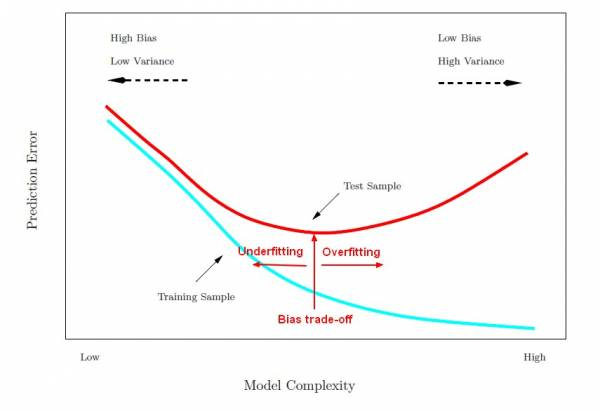
\includegraphics[width=0.45\textwidth]{figures/figure2.jpg}
\caption{Generalization Curve}
\end{center}
\end{figure}

\newpage

\section{Choosing the Training and Validation Sets}

In R the function \texttt{sample()} can be used to select indices of observations we want to include in either set. It is important to use random sampling to avoid orderings inherent to the dataset, thus avoiding trends that affect the bias of the models. It is also important, however, to use as much of the dataset as possible in order to arrive at a model with the greatest predictive power. One solution is to use K-fold cross validation, which involves using different subsets of the training and validation data so that each observation is part of the validation at least one. Then, average across all the runs to find the best predictive model. 

\begin{figure}[h]
\begin{center}
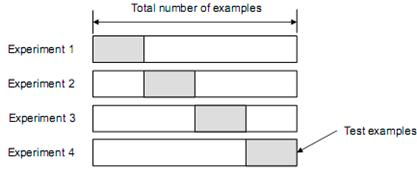
\includegraphics[width=0.5\textwidth]{figures/figure3.jpg}
\caption{K-Folds Cross Validation with K = 4}
\end{center}
\end{figure}

\section{Regularization}

Regularization penalizes complexity in the loss function for a specific choice to map it in the model. Do so by using Ridge Regularization or Lasso Regularization. 

\subsection*{Ridge Regularization}

$$\mathcal{L}=\frac{1}{n}\sum_i^n(y_i-wx_i)^2+\lambda \vert\vert w\vert\vert^2$$

As $\lambda$ increases, the coefficient decrease. This reduces the weighting of the model fit.

\subsection*{Lasso Regularization}

$$\mathcal{L}=\frac{1}{n}\sum_i^n(y_i-wx_i)^2+\vert\vert w_1\vert\vert+\vert\vert w_2\vert\vert+...$$

This performs variable selection by ignoring coefficients that are near zero.






\end{document}

%%% Local Variables:
%%% mode: latex
%%% TeX-master: t
%%% End:
